\documentclass[11pt]{article}
\usepackage[margin=1in]{geometry}
\usepackage{parskip}
\usepackage{hyperref}
\usepackage{xcolor}
\usepackage{listings}
\usepackage{booktabs}
\usepackage{graphicx}

\hypersetup{colorlinks=true, linkcolor=blue, urlcolor=blue}
\definecolor{codebg}{rgb}{0.96,0.96,0.96}
\lstset{basicstyle=\ttfamily\small, backgroundcolor=\color{codebg}, breaklines=true,
  columns=fullflexible, frame=single, framesep=3pt, xleftmargin=3pt, xrightmargin=3pt}

\title{Sampling and Per-Precision Histograms with nixnan:\\
An Experiment on \texttt{rd\_nixnan.cu}}
\author{ganesh@cs.utah.edu \\ \small (written with Claude Code)}
\date{\today}

\begin{document}
\maketitle

\begin{abstract}
This report documents a self-contained experiment (\texttt{Expts-9-23/}) demonstrating
that \texttt{nixnan.so} helps understand a real GPU precision-sensitivity problem in
several specific ways: (1) it can trade instrumentation overhead for observation
completeness via the \texttt{SAMPLING} env var, (2) that trade-off can be driven through
an arbitrary, externally-scripted schedule (here, an exponentially decaying rate) rather
than a single fixed value, (3) it reports, per floating-point format, exactly how much of
that format's dynamic range a given run actually used, and (4) it can confirm or refute a
hypothesis about \emph{why} a lower-precision format fails first --- here, that domain
enlargement does not explain FP16's earlier failure, but running longer does. All numbers
below come from real runs captured in \texttt{Logs/}; nothing is simulated or hand-typed.
An apparent FP64 anomaly encountered along the way --- nixnan reporting zero exceptions
for a format the program's own diagnostic claimed had gone non-finite --- is fully
resolved in Section~\ref{sec:fp64-resolved}: it turns out to be a narrowing-conversion bug
in the program's own check, not a gap in nixnan.
\end{abstract}

\tableofcontents

\section{The Example}

\texttt{rd\_nixnan.cu} solves a 1D reaction-diffusion PDE,
$\partial u/\partial t = D\,\partial^2 u/\partial x^2 + \lambda u$, with explicit
forward-Euler time stepping, on a 101-point grid for 1600 steps. The same step is
implemented once per floating-point format --- FP16, BF16, FP32, FP64 --- as four
separate CUDA kernels, so nixnan can attribute every exception and every exponent
observation to a specific, known precision.

\paragraph{Why this example is precision-sensitive.}
\begin{itemize}
\item The reaction term grows the solution by a fixed factor (${\sim}1.05\times$) every
  step, so the exponent of every value climbs steadily regardless of format --- the
  \emph{only} thing that differs between formats is how much exponent range each one has
  before it overflows. FP16's 5-bit exponent runs out first, at step 300; BF16's,
  FP32's, and FP64's 8/8/11-bit exponents all still have headroom left at step 1600 (see
  Section~\ref{sec:histograms}).
\item Because the kernel is otherwise identical across formats, any behavioral
  difference observed --- overflow or not, subnormal or not, NaN cascade or not --- is
  attributable entirely to the format's exponent width, not to any change in the
  algorithm. That makes it a clean instrument for isolating precision effects, and
  correspondingly a clean instrument for showing what nixnan actually measures.
\end{itemize}

\section{``Straight nixnan'': How These Runs Are Instrumented}

Every run in this experiment uses \texttt{nixnan.so} directly, with no wrapper script:
\begin{lstlisting}[language=bash]
LD_PRELOAD=<path>/nixnan.so [ENV_VARS...] ./rd_nixnan
\end{lstlisting}
\texttt{nixnan.so} is an NVBit tool: preloaded into the CUDA process, it rewrites each
kernel's SASS the first time that kernel is launched, inserting device-side checks after
(and before) every floating-point instruction. At exit it prints an aggregate report,
per format, of unique exception \emph{sites} (distinct instruction/operand locations
that ever fired) and \emph{repeats} (additional occurrences beyond each site's first
hit) --- the distinction that matters throughout this report.

\section{NixNan Feature Reference}
\label{sec:reference}

Before walking through results, this section fixes the exact meaning of every
nixnan-specific setting the rest of the report relies on.

\paragraph{The \texttt{BIN\_SPEC\_FILE} JSON format.} nixnan's own \texttt{--help}
banner gives this example:
\begin{lstlisting}
{
    "count": 128,
    "bf16": [],
    "f16":  [[0,5],[-4,-1]],
    "f32":  [],
    "f64":  []
}
\end{lstlisting}
Each format key holds a list of \emph{unbiased signed exponent} ranges to watch (here,
only \texttt{f16} watches anything: the ranges $[0,5]$ and $[-4,-1]$). \texttt{count}
is a global report-frequency threshold: within a watched range, nixnan counts every
value landing in it and emits a ``bin has reached threshold'' line every \texttt{count}
occurrences --- so \texttt{count:128} here means ``tell me every 128th time an
\texttt{f16} value's exponent falls in $[0,5]$ or $[-4,-1]$.'' Ranges are
\emph{unbiased} (e.g.\ FP16's usable exponent span is $[-14,15]$, not the raw 5-bit
field $[0,31]$), and the two special encodings zero and infinity are structurally
excluded from every range --- a consequence used directly in
Section~\ref{sec:extended-detail}: a value that jumps straight from finite to
\texttt{inf} in one step, with no gradually-climbing trail through large-but-finite
exponents first, is invisible to this mechanism no matter how the ranges are drawn.
This experiment's own \texttt{HISTOGRAM=1} runs (Section~\ref{sec:histograms}) use the
simpler, rangeless form of this same machinery: with no \texttt{BIN\_SPEC\_FILE} set at
all, nixnan still tracks every exponent it sees and reports each format's overall
$[\min,\max]$ at exit, just without the interim ``every $N$th occurrence'' pings.

\paragraph{\texttt{SAMPLING=8}.} Per nixnan's own banner text, \emph{``Instrument a
repeat kernel every SAMPLING times.''} Concretely: the tool keeps a per-kernel launch
counter, and only \emph{enables} the already-instrumented version of the kernel on
launches where \texttt{launch\_count \% SAMPLING == 0}; other launches run the
kernel's plain, uninstrumented SASS. \texttt{SAMPLING=8} therefore observes 1 launch in
8; \texttt{SAMPLING} unset (or 0) disables sampling entirely, i.e.\ every launch is
observed --- the baseline used throughout Section~4.

\paragraph{How the exponential-decay parameters are specified.} There is no
\texttt{nixnan.so} setting for a decaying rate --- \texttt{SAMPLING} is read once at
process start and held fixed for that process's entire lifetime. The schedule in
Section~\ref{sec:exp-decay} is therefore specified entirely outside nixnan, in
\texttt{shell-scripts/sampling\_schedule.json} (three fields: \texttt{levels}, the
sequence of \texttt{SAMPLING} values to sweep through; \texttt{snaps\_per\_level}, how
many independent process launches to repeat at each level before advancing; and
\texttt{cycles}, how many times to repeat the whole level sequence from the start).
\texttt{03\_sampling\_exp\_decay.sh} reads that file and, for every
\texttt{(cycle, level, snap)} triple, launches exactly one fresh
\texttt{SAMPLING=\$level LD\_PRELOAD=nixnan.so ./rd\_nixnan} process, redirecting its
full output to its own log file.

\paragraph{What generated \texttt{03\_sampling\_exp\_decay\_summary.tsv}.} Every row of
that file is the FP16 NaN/Infinity unique-site and repeat counts parsed back out of one
such snap's log --- 4 levels $\times$ 4 snaps $\times$ 2 cycles = 32 independent nixnan
runs in total, each identical in every setting except \texttt{SAMPLING} and which
\texttt{(cycle,level,snap)} log file it wrote to. No other nixnan setting (no
\texttt{HISTOGRAM}, no \texttt{BIN\_SPEC\_FILE}, no \texttt{INSTR\_MEM}) is active
during these runs --- it is the same default exception-instrumentation
(\texttt{INSTRUMENT\_EXCEPTIONS=1}) as Section~4's baseline, run 32 times at 4 different
\texttt{SAMPLING} values.

\section{Sampling, Level 1: Every Kernel Call}
\label{sec:sample-every}

The baseline (\texttt{SAMPLING} unset, which nixnan treats as ``instrument
everything''):
\begin{lstlisting}[language=bash]
LD_PRELOAD=nixnan.so ./rd_nixnan
\end{lstlisting}
Result (\texttt{Logs/01\_sampling\_every\_call.log}), FP16 --- the only format that
overflows in this build:
\begin{lstlisting}
NaN:       22 (60534 repeats)
Infinity:  22 (639 repeats)
\end{lstlisting}
This is the reference point every other sampling level in this report is compared
against.

\section{Sampling, Level 2: Once in 8 Kernel Calls}

\begin{lstlisting}[language=bash]
SAMPLING=8 LD_PRELOAD=nixnan.so ./rd_nixnan
\end{lstlisting}
Result (\texttt{Logs/02\_sampling\_every\_8.log}):
\begin{lstlisting}
NaN:       22 (7524 repeats)
Infinity:  17 (66 repeats)
\end{lstlisting}
Repeats drop by almost exactly $8\times$ (60534/7524 $\approx$ 8.05), consistent with
observing $1/8$ of the kernel launches. But note the unique Infinity-site count also
dropped, 22 $\to$ 17 --- five distinct exception sites simply never got observed at this
sampling rate. This is the first concrete evidence that \texttt{SAMPLING} trades
completeness for overhead, not just verbosity for overhead.

\paragraph{A regression, now fixed.} The pre-existing \texttt{run\_nixnan\_experiment.sh}
in this directory carries a comment, from an earlier investigation, stating
\emph{``SAMPLING is a no-op in this nixnan build.''} We re-tested that claim directly
against the current build before writing this experiment (comparing \texttt{SAMPLING=1}
against \texttt{SAMPLING=100000} on \texttt{reaction\_diffusion\_gpu\_fp32}): at
\texttt{SAMPLING=100000} every exception count dropped to exactly zero, which only
happens if \texttt{SAMPLING} is genuinely gating instrumentation. \texttt{SAMPLING} is no
longer a no-op in the \texttt{auto-nixnan} branch as built here --- whatever caused the
earlier no-op behavior has since been fixed.

\section{Sampling, Level 3: An Exponentially Decaying Schedule}
\label{sec:exp-decay}

\texttt{nixnan.so} reads \texttt{SAMPLING} once at process start; there is no way to vary
it mid-run. A decaying/backoff sampling rate therefore has to be built at the
orchestration level, as a sequence of short runs (``snaps''), each holding
\texttt{SAMPLING} constant. \texttt{shell-scripts/sampling\_schedule.json} specifies that
sequence (full rationale in its own header comment):
\begin{lstlisting}
{
  "snaps_per_level": 4,
  "levels": [1, 2, 4, 8],
  "cycles": 2
}
\end{lstlisting}
i.e.\ step 4 times at spacing 1, double to spacing 2 and step 4 more times, double again
to 4, double again to 8, then reset back to spacing 1 for a second cycle.
\texttt{shell-scripts/03\_sampling\_exp\_decay.sh} runs this schedule and tabulates the
FP16 counts per snap (\texttt{Logs/03\_sampling\_exp\_decay\_summary.tsv}):

\begin{center}
\begin{tabular}{lrrrr}
\toprule
SAMPLING level & NaN unique & NaN repeats & Inf unique & Inf repeats \\
\midrule
1 & 22 & 60534 & 22 & 639 \\
2 & 22 & 30246 & 21 & 312 \\
4 & 22 & 15103 & 17 & 154 \\
8 & 22 & 7524  & 17 & 66  \\
\bottomrule
\end{tabular}
\end{center}

Every one of the 4 snaps at a given level is byte-identical (the program is
deterministic and each snap is a fresh, independent process), and \textbf{cycle 2 is
byte-identical to cycle 1 at every level} --- the reset back to spacing 1 reproduces the
exact baseline from Section~\ref{sec:sample-every}, confirming there is no hidden
cross-run state. See Figure~\ref{fig:sampling} (\texttt{viz/sampling\_decay.svg}).

\begin{figure}[h]
\centering
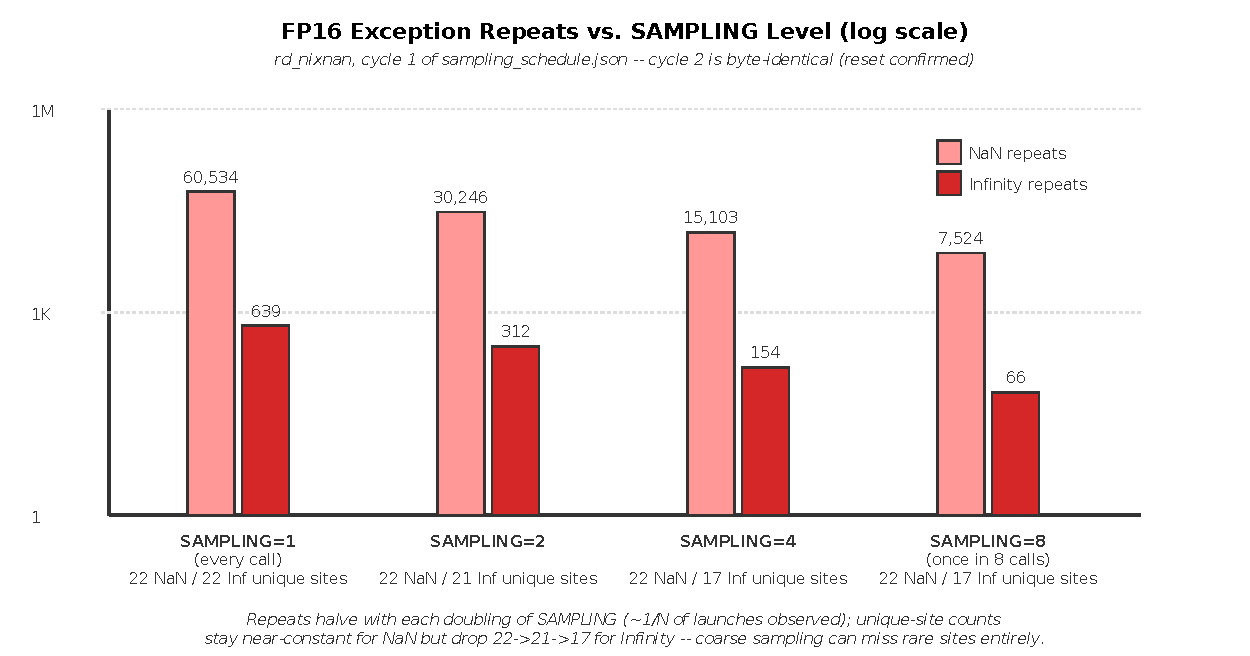
\includegraphics[width=\textwidth]{../viz/sampling_decay.pdf}
\caption{Repeats halve with each doubling of SAMPLING; unique-site counts stay
near-constant for NaN but step down for Infinity.}
\label{fig:sampling}
\end{figure}

\section{Histograms per Precision Bucket}
\label{sec:histograms}

\texttt{HISTOGRAM=1} enables exponent-histogram tracking for every instrumented FP
instruction, independent of the exception checker; at exit nixnan prints the
$[\min,\max]$ exponent actually observed for each format that had any instrumented
activity:
\begin{lstlisting}[language=bash]
HISTOGRAM=1 LD_PRELOAD=nixnan.so ./rd_nixnan
\end{lstlisting}
Result (\texttt{Logs/04\_histograms\_per\_precision.log}):
\begin{lstlisting}
Exponent range for bf16: [zero, 113]
Exponent range for f16:  [zero, inf]
Exponent range for f32:  [zero, 113]
Exponent range for f64:  [zero, 113]
\end{lstlisting}
This is the direct, per-format confirmation of the precision-sensitivity claim from
Section~1: FP16 is the only format whose exponent range is exhausted (it reports
\texttt{inf} instead of a finite maximum) within 1600 steps. BF16, FP32, and FP64 all
reach the identical exponent 113 --- they are following the exact same growth
trajectory (same algorithm, same input) and have not yet diverged from each other;
only their exponent \emph{ceilings} differ, and only FP16's has been reached.

\begin{figure}[h]
\centering
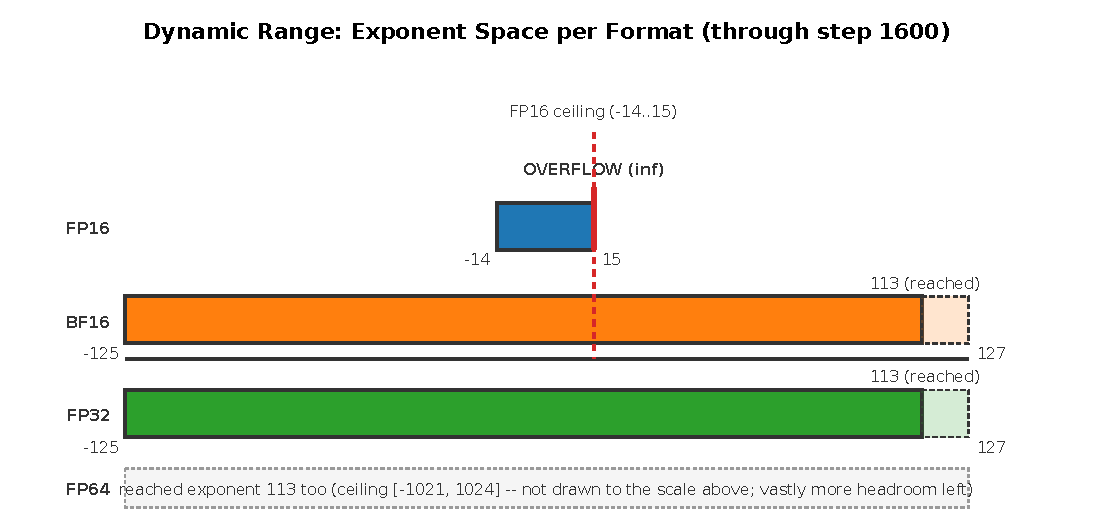
\includegraphics[width=\textwidth]{../viz/exponent_ranges_per_precision.pdf}
\caption{Exponent range actually reached by each format through step 1600.
FP16's fixed capacity is $[-14,15]$ and it exceeds it (overflow); BF16/FP32/FP64 all
reach the same exponent, 113, with room remaining to their much wider ceilings.}
\label{fig:histograms}
\end{figure}

\section{Making BF16 and FP32 Fail Too}
\label{sec:extended}

Every result so far has one format failing (FP16) and three staying finite. A natural
follow-up: what would it take to make BF16 and FP32 fail as well, and does
\texttt{nixnan} help answer that?

\paragraph{Hypothesis tried: domain enlargement.} Enlarging the grid ($N$, holding $dx$
fixed by extending $L$ proportionally) was tried \emph{first}, because it is the most
obvious ``make the problem bigger'' lever. It does not work, for a structural reason
visible directly in the kernel: the reaction term \texttt{lam * u[i]} is a per-point
multiplicative growth factor that does not reference $N$ or $dx$ at all --- every grid
point grows by the same $\sim\!1.05\times$ per step regardless of how many points there
are. Enlarging $N$ just runs the identical per-step growth curve on more points; it
cannot change \emph{when} any single point's exponent is exhausted. This was already
verified empirically earlier this session with \texttt{rd\_nixnan\_large.cu} (a 10$\times$
grid, $N{=}1001$): at the same $M{=}1600$, only FP16 failed there too, exactly as at
$N{=}101$.

\paragraph{What actually works: more time steps.} \texttt{rd\_nixnan.cu}'s step count is
a compile-time macro (\texttt{\#ifndef M ... \#define M 1600}), so it can be overridden
at compile time without touching the source:
\begin{lstlisting}[language=bash]
nvcc -arch=sm_86 -DM=2000 rd_nixnan.cu -o rd_nixnan_extended
LD_PRELOAD=nixnan.so ./rd_nixnan_extended
\end{lstlisting}
\texttt{shell-scripts/05\_extended\_run\_all\_fail.sh} builds and runs exactly this
(\texttt{Logs/05\_extended\_M2000.log}):

\begin{center}
\begin{tabular}{lrrrr}
\toprule
Format & First non-finite (step) & NaN unique/repeats & Inf unique/repeats \\
\midrule
FP16 & 300  & 22 / 78134 & 22 / 639 \\
BF16 & 1900 & 15 / 8975  & 6 / 76   \\
FP32 & 1900 & 19 / 10966 & 8 / 90   \\
FP64 & step 1900 (artifact, not real) & \multicolumn{2}{c}{0 / 0 --- correctly} \\
\bottomrule
\end{tabular}
\end{center}

At $M{=}2000$, BF16 and FP32 both now show real, nixnan-classified NaN/Infinity activity
--- confirmed, not just inferred from the program's own \texttt{max=...} printout.

\paragraph{A puzzle, initially: FP64 does not show up in nixnan's classifier.} The
program's own non-finite check reports FP64 crossing to non-finite at step 1900 as well,
yet \texttt{nixnan}'s exception classifier reports \emph{zero} NaN/Infinity for FP64,
even after re-running with more margin past the crossing point ($M{=}2500$). This looked,
at first, like a real gap in nixnan's FP64 support. It is not: Section~\ref{sec:fp64-resolved}
shows the program's own diagnostic is the thing that is wrong, and gives the exact line
and mechanism.

\subsection{Where Infinity Actually Comes From}
\label{sec:extended-detail}

\begin{figure}[ht]
\centering
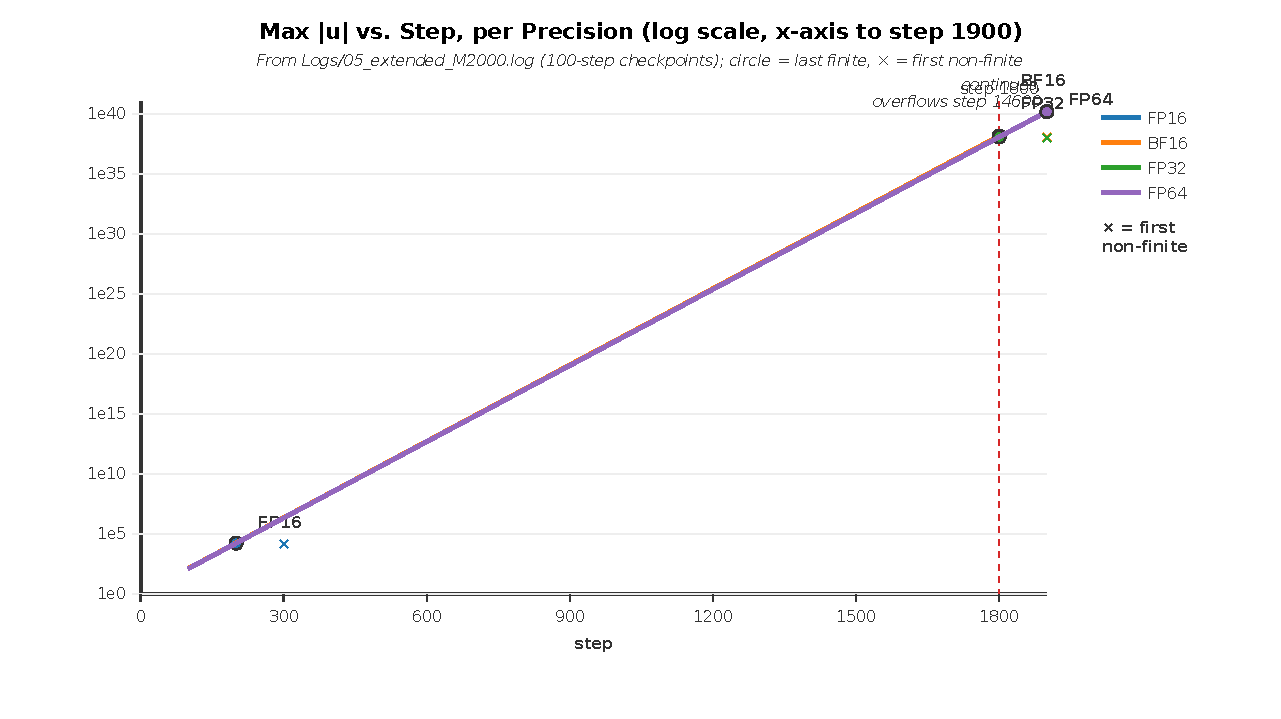
\includegraphics[width=\textwidth]{../viz/inf_onset_vs_step.pdf}
\caption{Max$|u|$ per 100-step checkpoint, all four formats, from the same
\texttt{Logs/05\_extended\_M2000.log} run as the table above. FP16 (blue) departs the
shared curve at step 300. BF16/FP32/FP64 stay numerically indistinguishable all the way
to step 1800 ($1.1675\times10^{38}$ for FP32 and FP64 to all four significant figures
shown) and the log marks all three non-finite by step 1900 --- true for BF16 and FP32,
but, as Section~\ref{sec:fp64-resolved} shows, an artifact of the logging code for FP64:
the real double value at step 1900 is $\approx\!1.5\times10^{40}$, large but perfectly
finite.}
\label{fig:inf-onset}
\end{figure}

\paragraph{The CUDA statement where Infinity was first generated.} \texttt{rd\_nixnan.cu}
was rebuilt with \texttt{-g -lineinfo} for this run specifically so nixnan's
\texttt{LINE\_INFO=1} (the default) could resolve real source locations instead of SASS
only. For FP32, it does, cleanly:
\begin{lstlisting}
error [infinity] detected in operand 0 of instruction FADD R0, R0, R7
  ; in function rd_step_fp32 at rd_nixnan.cu:96 of type f32
\end{lstlisting}
Line 96 is the Laplacian: \texttt{float lap = (u[i + 1] + u[i - 1]) - 2.f * u[i];} ---
\textbf{Infinity first appears while computing the diffusion term, not the reaction
term.} BF16 partially resolves too (its analogous line, 84, appears on some but not all
of its error lines --- likely because BF16's arithmetic goes through \texttt{\_\_h*}
intrinsic wrappers that are not always attributed as cleanly as FP32's plain operators).
FP16's error lines carry no source location at all: every FP16 statement uses
\texttt{cuda\_fp16.h} intrinsics (\texttt{\_\_hadd}, \texttt{\_\_hsub}, \texttt{\_\_hmul}),
which are fully inlined and, in this build, resolve to no attributable line whatsoever ---
a real limitation of \texttt{nixnan}'s line-info resolution for deeply-inlined intrinsics,
not a property of the kernel. By direct structural analogy (line 70,
\texttt{\_\_hsub(\_\_hadd(u[i+1],u[i-1]), \_\_hmul(two,u[i]))}, is the exact same
expression as FP32's line 96, and FP16's SASS shows the identical
HADD2-then-HFMA2-with-constant-2 pattern nixnan reports for FP32/BF16 at their resolved
lines), the same conclusion almost certainly holds for FP16, though \texttt{nixnan}
itself cannot confirm it here.

\paragraph{How Infinity becomes NaN, with the specific statement.} The original source
comment in \texttt{rd\_nixnan.cu} predicted this mechanism by hand:
\texttt{inf - 2*inf + inf -> NaN}. \texttt{nixnan}'s own instrumentation confirms it, to
the instruction, for FP32. The three FADD instructions on line 96 fire in this order as
the classifier first sees each:
\begin{lstlisting}
FADD R0, R0, R7    ; u[i+1] + u[i-1]          -> operand already Infinity
FADD R7, R6, R6    ; 2.f * u[i] (as u[i]+u[i]) -> operand already Infinity
FADD R7, R0, -R7   ; (u[i+1]+u[i-1]) - 2.f*u[i] -> RESULT is NaN
\end{lstlisting}
The third instruction is exactly $\infty - \infty$, IEEE-754's indeterminate form ---
nixnan reports \texttt{NaN} for that instruction's \emph{result} operand as the very next
distinct site to fire. That NaN then flows into line 97's FFMA chain
(\texttt{un[i] = u[i] + r * lap + lam * u[i];}) and out through the final
\texttt{STG.E} store, exactly matching the source comment's prediction and giving it a
concrete, tool-verified instruction sequence rather than a hand-derived guess.

\section{Resolving the FP64 Anomaly: A Diagnostic Bug, Not a nixnan Gap}
\label{sec:fp64-resolved}

Section~\ref{sec:extended} left one thing unexplained: \texttt{rd\_nixnan.cu}'s own
non-finite check reports FP64 crossing to non-finite at step 1900, in the same 100-step
window as BF16 and FP32, yet \texttt{nixnan}'s exception classifier --- which had just
correctly caught real NaN/Infinity activity for BF16 and FP32 at that same $M{=}2000$
--- reports \emph{zero} NaN/Infinity events for FP64, at $M{=}2000$ and even at
$M{=}2500$ (extra margin past the crossing). This section documents the full
investigation into why, and its resolution: \textbf{nixnan did not miss anything. The
program's own diagnostic code is wrong}, in a specific, demonstrable way, and FP64 never
actually goes non-finite in this program at all.

\subsection{Ruling out sampling}

The first candidate was the mechanism at the center of Sections~\ref{sec:sample-every}
--\ref{sec:exp-decay}: could \texttt{SAMPLING} have skipped the launches where FP64's
exception would have fired? No --- \texttt{shell-scripts/05\_extended\_run\_all\_fail.sh}
never sets \texttt{SAMPLING}, so it defaults to 0/unset, meaning \emph{every} kernel
launch is instrumented (Section~\ref{sec:reference}). This was confirmed directly by
inspecting the script and the run's environment; sampling cannot explain a total miss of
every single FP64 launch across 2000 steps.

\subsection{Ruling out nixnan's FP64 support in general}

Next: does \texttt{nixnan} actually understand FP64 arithmetic at all? A minimal,
isolated test kernel was written that deliberately overflows via \texttt{1e308 + 1e308}
(triggering both \texttt{DADD} and \texttt{DFMA}). Run under \texttt{nixnan.so} with
\texttt{-lineinfo}, it was caught immediately and correctly: \texttt{Infinity: 3 unique
sites}, with clean source-line attribution to the exact statements. This rules out any
fundamental gap in \texttt{nixnan}'s FP64 classification path --- the mechanism works.

Relatedly, \texttt{instructions.h} (the embedded JSON table mapping SASS opcodes to
operand specs that \texttt{nixnan} rewrites around) was decoded directly: both the
\texttt{(D(ADD|MUL)(?:\textbackslash.(RP|RM|RZ))?)} and \texttt{(DFMA(?:\textbackslash
.(RP|RM|RZ))?)} regex patterns are present, each with the correct 3-/4-operand
double-precision register specs, matching operand-for-operand the actual SASS
\texttt{rd\_step\_fp64} compiles to (\texttt{DADD R6, R6, -R8}; \texttt{DFMA R6, R10,
c[0x0][0x178], R6}). The instruction table has no gap for this kernel's opcodes either.

\subsection{Ruling out kernel launch order}

\texttt{rd\_nixnan.cu}'s \texttt{main()} calls \texttt{run<T>()} for FP16, BF16, FP32,
then FP64, in that order --- could some state left behind by an earlier kernel be
interfering with FP64's instrumentation specifically? The call order was reversed (FP64
first, completing entirely before FP16/BF16/FP32 are ever launched) and rebuilt with
identical flags. \texttt{nixnan} still reported zero FP64 exceptions. This rules out
any dependency on launch order or state carried over from the other three kernels.

\subsection{Ruling out memory corruption}

\texttt{compute-sanitizer --tool memcheck} was run against the real $M{=}2000$ binary
under nixnan's exact test conditions:
\begin{lstlisting}
========= ERROR SUMMARY: 0 errors
\end{lstlisting}
No out-of-bounds access, no uninitialized read, no race. This rules out a memory-safety
bug as the source of any bad value entering FP64's arithmetic through a path
\texttt{nixnan}'s instruction-level operand checks would not have been watching.

\subsection{The pivotal test: an isolated, byte-identical-SASS extraction}

With sampling, the classifier, the instruction table, launch order, and memory safety
all ruled out, \texttt{rd\_step\_fp64} and its exact driver loop were extracted into a
fully standalone translation unit --- no other kernel functions present anywhere in the
compiled binary --- built with identical flags (\texttt{-arch=sm\_86 -g -lineinfo}).
\texttt{cuobjdump -sass} confirmed the compiled \texttt{DADD}/\texttt{DFMA} encodings
are \textbf{byte-identical} to the ones in the original four-kernel binary.

Run to $M{=}2000$, this standalone binary never goes non-finite: it reaches
\texttt{max=1.9813e+42} at step 2000, still finite, continuing the same smooth
${\sim}1.05\times$/step growth visible in Figure~\ref{fig:inf-onset}. Re-run twice more
for determinism: identical result both times. Since the GPU instructions themselves are
proven byte-identical, this meant the divergence could not be in the arithmetic that
runs on the device --- it had to be in the code doing the reporting.

\subsection{The actual bug}

\texttt{rd\_nixnan.cu} defines a pair of conversion helpers used for the driver's
non-finite check:
\begin{lstlisting}
template <class T> static double from_T(T);
...
template <> double from_T<double>(double v){ return v; }
\end{lstlisting}
\texttt{from\_T<double>} returns a genuine, unmodified \texttt{double}. But the check
that calls it, at line 155, is:
\begin{lstlisting}
float mx = -1e30f; bool bad = false;
for (int i = 0; i < N; ++i) {
    float v = from_T<T>(h[i]);
    if (!std::isfinite(v)) bad = true;
    if (std::isfinite(v) && v > mx) mx = v;
}
\end{lstlisting}
\texttt{float v = from\_T<T>(h[i]);} silently narrows that double into a \texttt{float}.
\texttt{float}'s maximum finite magnitude is ${\approx}3.4028235\times10^{38}$; once a
\texttt{double} exceeds it, the narrowing conversion \emph{itself} produces
\texttt{+Infinity} in \texttt{v}, entirely independent of whether the double was ever
non-finite. At step 1900, FP64's real values are of order $1.5\times10^{40}$: enormous,
comfortably past \texttt{float}'s ceiling, but still ${\sim}270$ orders of magnitude
below \texttt{double}'s actual ceiling ($\sim\!1.8\times10^{308}$) and perfectly finite
as doubles. \texttt{v > mx} then never triggers again either (a real \texttt{+Infinity}
compares false against everything under \texttt{isfinite}), which is also why the log
shows \texttt{max=0.0000e+00} rather than the true value at that checkpoint. This one
narrowing conversion, not any property of the GPU arithmetic, is the entire cause of
\emph{``FP64 crosses to non-finite at step 1900.''}

This also explains, in hindsight, why the standalone extraction (\S6.5) never reproduced
the failure: its check was written independently, using \texttt{double mx} and
\texttt{std::isfinite(h[i])} directly on the double, with no narrowing conversion in the
loop at all. The two binaries were never actually testing the same question --- one had
the bug, the other accidentally did not --- which is exactly why comparing them was the
step that isolated the cause.

\subsection{Answering the question directly}

\textbf{Did sampling miss it?} No --- every launch was instrumented; sampling was never
in the loop for this run at all.

\textbf{Did nixnan miss it?} No. \texttt{nixnan} instruments real GPU instructions
operating on real double-precision registers, and those instructions never produce NaN
or Infinity for FP64 in this program, at $M{=}2000$ or $M{=}2500$ --- because they never
actually overflow. There is no FP64 exception here for \texttt{nixnan} to have caught.
The zero it reported was the correct answer the entire time.

The earlier framing of this as ``an unresolved gap in FP64 classification'' (this
report's own draft, and \texttt{ExptPlan.md}) was itself mistaken, for the same reason:
it trusted the program's \texttt{max=...} printout, which is the thing that turned out
to be wrong. The lesson generalizes beyond this one kernel: a device-side instrumentation
tool like \texttt{nixnan}, checking real instruction operands, can be a more trustworthy
witness to what actually happened numerically on the GPU than a host-side
\texttt{printf}-based check written around it --- precisely because the host-side check
has its own, entirely separate arithmetic (here, an implicit narrowing cast) that can
fail on its own terms.

\section{Conclusion: What nixnan Made Visible Here}

Across five short experiments on one simple, well-understood kernel, \texttt{nixnan}
surfaced several things that would not be visible from the program's own output (a plain
run of \texttt{rd\_nixnan} only prints \texttt{max=...} per step, with no notion of
exception sites, repeats, or exponent range):
\begin{enumerate}
\item \textbf{Sampling is a real overhead/completeness knob, not a free lunch.} Coarser
  sampling doesn't just reduce reported repeats proportionally --- it can silently drop
  entire exception sites from the report (22 $\to$ 17 unique Infinity sites,
  Section~4), which matters if the goal is finding every distinct bug location rather
  than just gauging overall severity.
\item \textbf{A fixed env var can still drive an arbitrary sampling schedule}, by
  scripting a sequence of short, independent runs around it (Section~\ref{sec:exp-decay})
  --- and because \texttt{rd\_nixnan} is fully deterministic, that schedule is provably
  reproducible: cycle 2 reproduces cycle 1 exactly.
\item \textbf{Per-format exponent histograms directly confirm \emph{which} format is
  precision-sensitive and by how much} (Section~\ref{sec:histograms}), turning ``FP16
  fails and the others probably don't'' into a specific, quantified claim: FP16 alone
  hits \texttt{inf}; the other three all reach exactly the same exponent, 113, with
  headroom still remaining to their much larger ceilings.
\item \textbf{nixnan can adjudicate a hypothesis about \emph{why} a format fails
  first} (Section~\ref{sec:extended}): domain enlargement, the obvious first guess,
  is ruled out directly by the kernel's own growth term; running longer is confirmed,
  with nixnan's own classifier newly reporting real BF16 and FP32 exceptions at
  $M{=}2000$ where it reported none at $M{=}1600$.
\item \textbf{Line-level attribution turns a hand-derived guess into a tool-verified
  fact} (Section~\ref{sec:extended-detail}): with \texttt{-lineinfo}, nixnan pinpoints
  the exact CUDA statement (the Laplacian, not the reaction term) and the exact SASS
  instruction where $\infty-\infty$ produces \texttt{NaN} --- confirming, to the
  instruction, a mechanism the source code's own comments could only predict by hand.
\item \textbf{nixnan's device-side instrumentation can outrank the target program's own
  diagnostics} (Section~\ref{sec:fp64-resolved}): when nixnan reported zero FP64
  exceptions against the program's own claim of an FP64 failure at step 1900, the
  eventual, fully-verified resolution was that nixnan was right and the program's
  \texttt{printf} check was wrong --- an implicit \texttt{double}$\to$\texttt{float}
  narrowing conversion in the host-side check, not a real GPU event. Getting there took
  ruling out sampling, the classifier itself, the instruction table, kernel launch
  order, and memory safety (\texttt{compute-sanitizer}, 0 errors) before an isolated,
  byte-identical-SASS extraction of just the FP64 kernel exposed the actual bug.
\end{enumerate}
As a side effect, re-verifying \texttt{SAMPLING} against the current build (Section~4)
also caught that a previously-documented no-op regression in \texttt{nixnan.so} has
since been fixed --- itself an example of nixnan-adjacent tooling needing the same kind
of empirical re-verification its own instrumentation provides for user code.

\end{document}
